\documentclass[12pt]{article}
\usepackage[margin=2.5cm]{geometry}
\usepackage{enumerate}
\usepackage{amsfonts}
\usepackage{amsmath}
\usepackage{fancyhdr}
\usepackage{amsmath}
\usepackage{amssymb}
\usepackage{amsthm}
\usepackage{mdframed}
\usepackage{graphicx}
\usepackage{subcaption}
\usepackage{adjustbox}
\usepackage{listings}
\usepackage{xcolor}
\usepackage{booktabs}
\usepackage[utf]{kotex}
\usepackage{hyperref}
\usepackage{accents}

\definecolor{codegreen}{rgb}{0,0.6,0}
\definecolor{codegray}{rgb}{0.5,0.5,0.5}
\definecolor{codepurple}{rgb}{0.58,0,0.82}
\definecolor{backcolour}{rgb}{0.95,0.95,0.92}

\lstdefinestyle{mystyle}{
    backgroundcolor=\color{backcolour},
    commentstyle=\color{codegreen},
    keywordstyle=\color{magenta},
    numberstyle=\tiny\color{codegray},
    stringstyle=\color{codepurple},
    basicstyle=\ttfamily\footnotesize,
    breakatwhitespace=false,
    breaklines=true,
    captionpos=b,
    keepspaces=true,
    numbers=left,
    numbersep=5pt,
    showspaces=false,
    showstringspaces=false,
    showtabs=false,
    tabsize=1
}

\lstset{style=mystyle}

\pagestyle{fancy}
\renewcommand{\headrulewidth}{0.4pt}
\lhead{CSC 343}
\rhead{Worksheet 8}

\begin{document}
\title{CSC343 Worksheet 8}
\maketitle

\begin{enumerate}[1.]
    \item \textbf{Exercise 9.5.1:} Repeat Exercise 9.3.1, but write the code using C with CLI calls.

    \bigskip

    \begin{enumerate}[a)]
        \item

        \bigskip

        \underline{\textbf{Notes:}}

        \begin{itemize}
            \item Using Call-Level Interface
            \begin{itemize}
                \item Uses host language to connect to and access a database
                \item Replaces embedded SQL
            \end{itemize}
            \item Standard SQL/CLI
            \begin{itemize}
                \item Is database CLI for C
                \item Included in file \textit{sqlcli.h}
                \item Creates deals with four kinds of records

                \bigskip

                \begin{enumerate}[1.]
                    \item Environment handle
                    \begin{itemize}
                        \item Prepares one or more connections to database server
                        \item Is required
                        \item \textbf{SQLHENV} does this job

                        \begin{center}
                        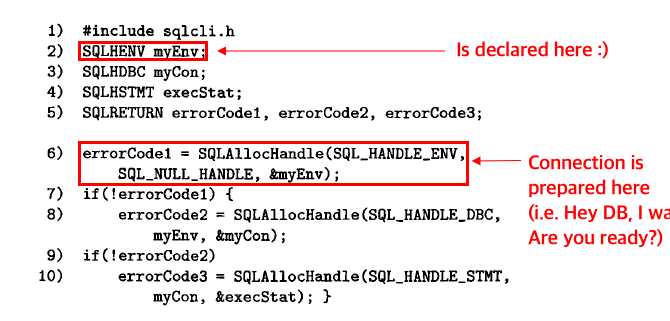
\includegraphics[width=\linewidth]{images/worksheet_8_solution_1.png}
                        \end{center}

                    \end{itemize}
                    \item Connection handle
                    \begin{itemize}
                        \item Connects to a data resource
                        \item Is required
                        \item Is declared after \textbf{SQLHENV}
                        \item \textbf{SQLHDBC} does this job
                    \end{itemize}
                    \item Statements
                    \item Descriptions
                \end{enumerate}
            \end{itemize}
            \item Processing Statements
            \item Fetching Data From
            \item Passing Parameters to Queries
        \end{itemize}

    \end{enumerate}


    \item \textbf{Exercise 9.5.2:} Repeat Exercise 9.3.2, but write the code using C with CLI calls
    \item \textbf{Exercise 9.6.1:} Repeat Exercise 9.3.1, but write the code using JAVA using JDBC.
    \item \textbf{Exercise 9.6.2:} Repeat Exercise 9.3.2, but write the code using JAVA using JDBC.
    \item \textbf{Exercise 9.7.1:} Repeat Exercise 9.3.1, but write the code using PHP.
    \item \textbf{Exercise 9.7.2:} Repeat Exercise 9.3.2, but write the code using PHP.
    \item \textbf{Exercise 9.7.3:} In Example 9.31 we exploited the feature of PHP that strings
    in double-quotes have variables expanded. How essential is this feature? Could
    we have done something analogous in JDBC? If so, how?
\end{enumerate}

\end{document}